\section{基本几何体三视图}
根据表面形状的不同可以将基本几何体分为平面立体和曲面立体。如果立体表面均由平面构成,则称为平面立体,如长方体、正方体、棱柱、棱锥、棱台等。如果立体表面由平面和曲面共同构成或全部由曲面构成,则称为曲面立体,如圆柱、圆球、圆环等。
\subsection{平面立体}
在平面立体中,其表面是由若干个平面多边形构成的,多边形的边是平面立体的轮廓线,是平面立体两个平面的交线,当轮廓的投影可见时,用粗实线表示;不可见时,用虚线表示;当实线与虚线重合时,应当用粗实线表示。
\subsubsection{棱柱体}
棱柱体由顶面、底面及若干个侧棱面构成。棱柱体的各个侧棱相互平行,顶面和底面相互平等。如果核柱的侧棱与顶面和底面垂直则称为直棱柱,否则称为斜棱柱。当直棱柱的顶面和底面为正多边形时则称为正棱柱。
\begin{figure}[htbp]
\centering
\subfloat[]{\label{fig:cube}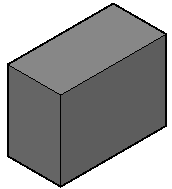
\includegraphics[scale=0.9]{cube.png}}\hspace{30pt}
\subfloat[]{\label{fig:cubethreeview}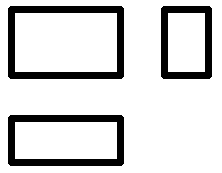
\includegraphics[scale=1]{cubethreeview.png}}
\caption{长方体的投影}
\end{figure}

图\ref{fig:cubethreeview}所示的长方体,其顶面与底面的水平投影重合并反映衬形,为一长方形,其它棱面的水平投影积聚为长方形的四条边;前面与后面的正投影重合并反映实形,顶面、底面和两个侧面积聚为长方形的四条件边;左面和右面的侧面投影重合并反映实形,顶面、底面、前面和后面积聚为长方形的四条件边。长方体的三视图投影如图\ref{fig:cube}所示。

图\ref{fig:sannenzhu}所示的正三棱柱,其顶面与底面的水平面投影重合并反映实形,为一正三角形。三个棱面在水平投影面积聚为三角形的三条边。三棱柱的三视图投影如图\ref{fig:sannenzhuthreeview}所示。
\begin{figure}[htbp]
\centering
\subfloat[]{\label{fig:sannenzhu}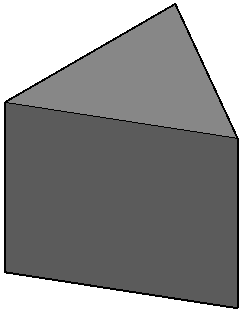
\includegraphics[scale=0.6]{sannenzhu.png}}\hspace{30pt}
\subfloat[]{\label{fig:sannenzhuthreeview}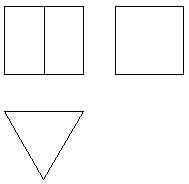
\includegraphics[scale=1]{sannenzhuthreeview.png}}
\caption{正三棱柱的投影}
\end{figure}

图\ref{fig:sixnenzhu}所示的正六棱柱,其顶面与底面的水平面投影重合并反映实形,为一正六边形。六个棱面在水平投影面积聚为六边形的六条边。正六棱柱的三视较长投影如图\ref{fig:sixnenthreeview}所示。
\begin{figure}[htbp]
\centering
\subfloat[]{\label{fig:sixnenzhu}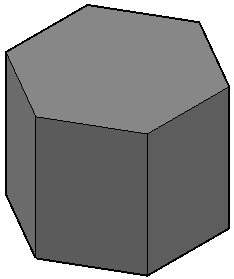
\includegraphics[scale=0.7]{sixnenzhu.png}}\hspace{30pt}
\subfloat[]{\label{fig:sixnenthreeview}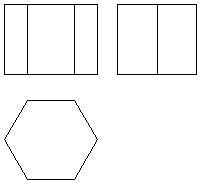
\includegraphics[scale=1]{sixnenthreeview.png}}
\caption{正六棱柱的投影}
\end{figure}

由此可见棱柱的投影特点是:一面投影反映底面实形,其余两面投影则为矩形或复合矩形。
\subsubsection{棱锥体}
棱锥体是由一个多边形底面和若干个共顶点的三角形棱面构成的。从棱锥体顶点到底面的垂直距离称为棱锥体的高。如果棱锥体的底面为正多边形,锥顶的投影位于多边形的中心,各棱面是等腰三角形,则该棱锥体称为正棱锥。正四棱锥的三面投影如图\ref{fig:fournenzhuithreeview}所示。

\begin{figure}[htbp]
\centering
\subfloat[]{\label{fig:fournengzhui}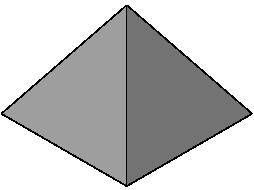
\includegraphics[scale=0.9]{fournengzhui.png}}\hspace{30pt}
\subfloat[]{\label{fig:fournenzhuithreeview}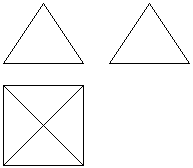
\includegraphics[scale=1]{fournenzhuithreeview.png}}
\caption{正四棱锥的投影}
\end{figure}

图\ref{fig:fournengzhui}所示的正四棱锥的底面与水平投影面平行,其投影反映实形,为正方形;底面在其它投影面积聚为一条直线;棱面的三面投影则为类似的三角形。

由此可见,棱锥体的投影特点是:一投影面为由三角形构成的复合多边形,其两投影为三角形或复合三角形。
\subsubsection{棱台体}
棱台体是由棱锥体被切掉顶部后所构成的一种形体。棱台体的投影特点是:一面投影为由梯形构成的内外相似复合多边形,其余两面投影则为梯形或复合梯形。图\ref{fig:fivenentai} 所示为五棱台的投影。
\begin{figure}[htbp]
\centering
\subfloat[]{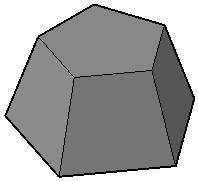
\includegraphics[scale=0.9]{fivenentai.png}}\hspace{30pt}
\subfloat[]{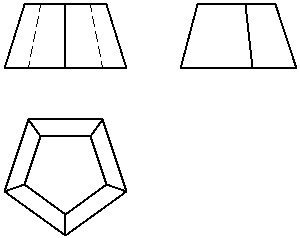
\includegraphics[scale=1]{fivenentaithreeview.png}}
\caption{五棱台的投影}\label{fig:fivenentai}
\end{figure}

\endinput